% !TEX program = pdflatex
% !BIB pro%gram = bibtex
% !TEX encoding = UTF-8 Unicode
% !TEX spellcheck = en_us
\documentclass[10pt,sigconf]{acmart}

\usepackage{booktabs} % For formal tables

\graphicspath{{figure/}{figures/}}

% Copyright
%\setcopyright{none}
%\setcopyright{acmcopyright}
%\setcopyright{acmlicensed}
\setcopyright{rightsretained}
%\setcopyright{usgov}
%\setcopyright{usgovmixed}
%\setcopyright{cagov}
%\setcopyright{cagovmixed}


% DOI
\acmDOI{10.475/123_4}

% ISBN
\acmISBN{123-4567-24-567/08/06}

%Conference
\acmConference[CR for Nano'21]{AzuNet Seminar}{July 2021}{Lübeck, Germany} 
\acmYear{2021}
\copyrightyear{2021}

\acmPrice{15.00}


\begin{document}
\title{Computational Requirements for Nano-machines}
\titlenote{Produces the permission block, and copyright information}
%\subtitle{Extended Abstract}

\author{Melanie Badura}
\orcid{1234-5678-9012}
\affiliation{%
  \institution{Universität zu Lübeck}
  \streetaddress{Ratzeburger Allee 160}
  \city{Lübeck}  
  \postcode{23560}
}
\email{melanie.badura@student.uni-luebeck.de}




% The default list of authors is too long for headers}
\renewcommand{\shortauthors}{F. Lastname et al.}


\begin{abstract}
This paper is a shortpaper for "Computational Requirements for 
Nano-Machines: There is limited Space at the bottom".\footnote{}
\end{abstract}

%
% The code below should be generated by the tool at
% http://dl.acm.org/ccs.cfm
% Please copy and paste the code instead of the example below. 
%
\begin{CCSXML}
<ccs2012>
 <concept>
  <concept_id>10010520.10010553.10010562</concept_id>
  <concept_desc>Computer systems organization~Embedded systems</concept_desc>
  <concept_significance>500</concept_significance>
 </concept>
 <concept>
  <concept_id>10010520.10010575.10010755</concept_id>
  <concept_desc>Computer systems organization~Redundancy</concept_desc>
  <concept_significance>300</concept_significance>
 </concept>
 <concept>
  <concept_id>10010520.10010553.10010554</concept_id>
  <concept_desc>Computer systems organization~Robotics</concept_desc>
  <concept_significance>100</concept_significance>
 </concept>
 <concept>
  <concept_id>10003033.10003083.10003095</concept_id>
  <concept_desc>Networks~Network reliability</concept_desc>
  <concept_significance>100</concept_significance>
 </concept>
</ccs2012>  
\end{CCSXML}


\ccsdesc[500]{Computer systems organization~Embedded systems}
\ccsdesc[300]{Computer systems organization~Redundancy}
\ccsdesc{Computer systems organization~Robotics}
\ccsdesc[100]{Networks~Network reliability}

% We no longer use \terms command
%\terms{Theory}

\keywords{ACM proceedings}


\maketitle

\section{Introduction}
For years, there has been talking of using nano-machines to create solutions for problems in medicine and other subjects. Such a machine should be able to communicate and sense/act. Computational power is also a big issue.
Because Nano-machines are small, one question is how to implement these capabilities. 
While many researchers already deal with communication technology (cite one here), computational capability is usually left out.
In this paper, there is an attempt to provide a general analysis of the computational capability of nano-machines.
Since the capabilities of nano-machines vary widely, from nanoparticles with no computational capabilities to microprocessors (11 cites). Nano-machines divide into three groups according to complexity theory,
by analyzing the tasks that nano-machines handle.



\section{Mittelteil?}
Most problems that a nano-machine has to solve need basic arithmetic.
Others are solved with pattern matching and parity.
To solve the communication problem, there are forwarding and routing protocols. 
These protocols are solved in different ways so that a nano-machine can handle several types of messages.
Communication is a perfect example for the use of basic arithmetics, pattern matching, storage needs.
However, not only for the storage of routing information they need memory but also for other values with which they must work, must be stored.
Nano-machines should also be able to perform more complex operations like implementing a neural network.
They use graph algorithms for this. 
All these problems divide into complexity classes.
As the name suggests, the problems divide into classes that have approximately the same complexity.
This is found out by reduction. For example, subtract can be reduced to add. 
Here, the simplest complexity class can be used, but also with a nano-machine that has been built to solve the problems of the most difficult complexity class.
However, this does not work the other way around.
In table \ref{table1}, the three different classes are seen.
An L-machine can solve problems like a Turing machine.
The class $AC^0$ describes boolean circuits with polynomial size and a constant depth, whereas the class $NC^1$ may have a logarithmic depth and two inputs per gate. 
\\
bla\\
bla\\bla\\
bla\\
bla\\bla\\
bla\\
bla\\bla\\
bla\\
bla\\bla\\
bla\\
bla\\bla\\
als nächstes ab 5 und du hast für mittelteil keinen titel und nicht geschaut was grammerly so sagt!
Das table kommt wieder wenn du hier mehr schreibt\\
\begin{table}
\begin{tabular}{ p{1.5cm}|p{2cm} p{2cm}|p{1.5cm} }
  \hline
  %\multicolumn{5}{|c|}{MSE} \\
  Machine & \multicolumn{2}{c|}{Problems}  & Origin\\
  \hline
  $AC^0$: & $ADD$ & $ODD/EVEN$&  \\
          & $SUB$ & $DIV_{2}$&  \\
          & $SIGN$ & $MOD_{2}$&  \\
          & $INC$ & $LOG_{2}$&  \\
          & $AND/OR$ & $INV$&  \\
          &  & &  \\
  $NC^1$:   & $MULT$ &$MIN/MAX$   & \\
           & $DIV$ & $PARITY$&  \\
           & $EXP$ & $REG$&  \\
           & $MAJOR$ & $MOD$&  \\
           & $THRES$ & $AVG$&  \\
           &  & &  \\
  $L$:      &   $Label$ &$D_{FS}$ &     \\
           & $Log mem$ & $B_{FS}$&  \\
           & $REACH$ & $MEDIAN$&  \\
          
  \hline 
  \end{tabular}\\
  
  \caption{Complexity classes of nano-machines}
  \label{table1}
  \end{table}
  


\section{Conclusion}

\subsection{Subsection}


\begin{figure}[htbp]
  \centering
  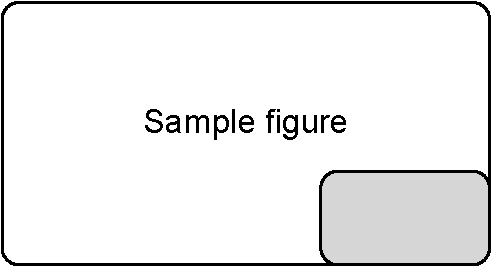
\includegraphics[scale=0.5]{sample-figure}
  \caption{Sample figure}
  \label{fig:sample}
\end{figure}




\bibliographystyle{acm}
\bibliography{sigproc} 

\end{document}
